\section{Representing personal data processing information}
\label{sec:sota_vocabularies}

The Web of Data and its semantic specifications are thriving, with the W3C guiding this effort to have machine-readable and interoperable linked data on the Web, described by open standards that promote portability and extensibility, allow for seamless integration of data from different origins and re-usage across distinct Web applications and services~\citep{berners-lee_semantic_2001}.
Accordingly, a wave of vocabularies and ontologies has appeared in the last few years to formalise common concepts, such as objects or entities, or terms from specific domains, such as legal or medical ontologies.
More recently, with the increasing concerns around personal data processing abuse by Big Tech companies, data protection has been on the agenda of governments in a worldwide manner, with the EU taking the lead with its data protection law, the GDPR.
This has led to a new wave of personal data protection law ontologies being developed to help companies comply with GDPR's legal requirements and which also intend to assist individuals in managing their personal data.

In the following Sections, the criteria used to analyse each specified data protection vocabulary are included, as well as a description of each identified solution.

\subsection{Criteria for analysis}
\label{sec:sota_vocabularies_criteria}

For each identified solution, we describe the core terms formalised in the ontologies, as well as dependencies on other existing works, and, when available, case studies where it has been applied.
As for the analysis of their representational abilities, we analyse whether such ontologies can represent the privacy terms mentioned in GDPR's data subject rights, to assess to what extent they can be used by data subjects to exercise their rights and by data controllers to manage compliance.

In particular, the so-called \textit{`right to be informed'}, described in detail in Articles 13 and 14, obliges data controllers to inform data subjects about any processing of personal data, whether being from data collected directly from the data subjects or from other sources. In addition to this, the following rights are also provided to data subjects:

\begin{enumerate}
  \item[(Art. 15)] \textit{`right of access'} to the personal data being processed, including a copy of the data as well as information about the purposes for processing, categories of the personal data being processed and their source, any recipients to whom the data may have been shared and corresponding measures to ensure its security, storage and retention conditions and the existence of other data subject's rights.
  \item[(Art. 16)] \textit{`right to rectification'} of inaccurate or incomplete personal data.
  \item[(Art. 17)] \textit{`right to be forgotten'}  by the data controllers when the personal data is no longer needed for the purposes for which it was collected.
  \item[(Art. 18)] \textit{`right to restriction of processing'} of personal data when its accuracy is being contested, the processing is unlawful, when the data subject needs it for any legal claims or objects to the processing.
  \item[(Art. 19)] \textit{`right to be notified'} about the rectification, erasure or restriction of processing.
  \item[(Art. 20)] \textit{`right to data portability'}, including the right to request that said data be transferred directly from one controller to another.
  \item[(Art. 21)] \textit{`right to object'} to any processing, including profiling.
  \item[(Art. 22)] \textit{`right to not be subjected to automated decision-making'}, including profiling.
\end{enumerate}

For such rights to be exercised by data subjects and fulfilled by data controllers, a set of privacy terms must be modelled, namely the terms identified in Table~\ref{tab:GDPR_privacy_terms}, which is derived from~\cite{esteves_analysis_2022}. These terms will be used to compare the described privacy and data protection vocabularies and ontologies and identify representational gaps in the existing solutions. The outcomes of this comparative analysis will be provided in Section~\ref{sec:sota_vocabularies_analysis}.

\begin{table}[htp]
\centering
\caption{Privacy terms to be represented and respective identifiers (I*). The GDPR articles that mention these terms are also specified.}
\label{tab:GDPR_privacy_terms}
\resizebox{\textwidth}{!}{%
\begin{tabular}{c||l|c}
 I* & Informational Items & \textbf{GDPR Article(s)} \\
 \hline\hline
 I1 & Controller identity & \textbf{13.1(a), 14.1(a)} \\
 \hline
 I2 & Controller contact details & \textbf{13.1(a), 14.1(a)} \\
 \hline
 I3 & Controller's representative identity & \textbf{13.1(a), 14.1(a)} \\
 \hline
 I4 & Controller's representative contact details & \textbf{13.1(a), 14.1(a)} \\ 
 \hline
 I5 & DPO contact details & \textbf{13.1(b), 14.1(b)} \\
 \hline
 I6 & Purposes of the processing & \textbf{13.1(c), 14.1(c), 15.1(a)} \\ 
 \hline
 I7 & Legal basis of the processing & \textbf{6.1, 9.2, 13.1(c), 14.1(c)} \\ 
 \hline
 I8 & Legitimate interests & \textbf{6.1(f), 13.1(d), 14.2(b)} \\ 
 \hline
 I9 & Recipients / categories of recipients & \textbf{13.1(e), 14.1(e), 15.1(c), 17.2, 19} \\
 \hline
 I10 & Transfers to third countries & \textbf{13.1(f), 14.1(f)} \\ 
 \hline
 I11 & Retention period & \textbf{13.2(a), 14.2(a), 15.1(d)} \\ 
 \hline
 I12 & Data subject's rights & \textbf{13.2(b), 14.2(c), 15.1(e)} \\ 
 \hline
 I13 & Right to withdraw consent & \textbf{6.1(a), 9.2(a), 13.2(c), 14.2(d)} \\ 
 \hline
 I14 & Right to lodge a complaint & \textbf{13.2(d), 14.2(e), 15.1(f)} \\ 
 \hline
 I15 & Statutory or contractual obligation details & \textbf{13.2(e)} \\ 
 \hline
 I16 & Existence of automated decision making & \textbf{13.2(f), 14.2(g), 15.1(h), 22.1, 22.4} \\ 
 \hline
 I17 & Categories of personal data & \textbf{9.1, 14.1(d), 15.1(b)} \\ 
 \hline
 I18 & Source of personal data & \textbf{14.2(f), 15.1(g)} \\ 
 \hline
 I19 & Grounds to not comply with information right & \textbf{13.4, 14.5} \\
 \hline
 I20 & Safeguards related to the transfer to a third country & \textbf{15.2} \\ 
 \hline
 I21 & Copy of personal data & \textbf{15.3, 20.1} \\ 
 \hline
 I22 & Request to complete incomplete personal data & \textbf{16} \\ 
 \hline
 I23 & Grounds to request erasure of data & \textbf{17.1} \\ 
 \hline
 I24 &  Technical measures taken to erase data & \textbf{17.2} \\
 \hline
 I25 & Recipients contact details & \textbf{17.2, 19} \\
 \hline
 I26 & Grounds to not comply with right of erasure & \textbf{17.3} \\
 \hline
 I27 & Grounds to request restriction of processing & \textbf{18.1} \\
 \hline
 I28 & Transfer data directly between controllers & \textbf{20.2} \\
 \hline
 I29 & Grounds to not comply with right to object & \textbf{21} \\
 \hline
 I30 & \multicolumn{1}{l|}{\begin{tabular}[l]{@{}l@{}} Grounds to not comply with right not to be \\ subjected to decision making \end{tabular}} & \textbf{22.2} \\
\end{tabular}}
\end{table}

\subsection{Personal data protection vocabularies}
\label{sec:sota_vocabularies_description}

In this Section, a systematic description of each identified work is provided, including an example that uses the vocabulary's concepts, when available.
Moreover, Table~\ref{tab:analysed_vocabularies} provides an overview of these solutions and supplies information about the creators of the resources, their versions, the date of publication, and the date of the last known update.
Said solutions are then analysed in chronological order regarding the date of publication and a dependency graph -- a chart that demonstrates the relations between the reviewed vocabularies and its dependencies and extensions -- is presented in Figure~\ref{fig:voc_dependency_graph}.

\begin{table}[ht]
\centering
\caption{Brief description of the vocabularies described in Section \ref{sec:sota_vocabularies_description}.}
\label{tab:analysed_vocabularies}
\resizebox{\textwidth}{!}{%
\begin{tabular}{c||c|c|c|c|c}
Abbreviation (Section) & Full Name & Creators & Version & \multicolumn{1}{c|}{\begin{tabular}[c]{@{}c@{}} Date of \\ publication \end{tabular}} & \multicolumn{1}{c}{\begin{tabular}[c]{@{}c@{}} Last \\ update \end{tabular}} \\
 \hline\hline
 \multicolumn{1}{c||}{\begin{tabular}[c]{@{}c@{}} DPKO, \\ DPRO (\ref{sec:neurona}) \end{tabular}} & \multicolumn{1}{c|}{\begin{tabular}[c]{@{}c@{}} Data Protection Knowledge Ontology, \\ Data Protection Reasoning Ontology \end{tabular}} & Casellas et al. & - & 2008 & 2010 \\
 \hline
 DPO (\ref{sec:dpo}) & Data Protection Ontology & Bartolini and Muthuri & - & 2015 & 2016 \\
 \hline
 GDPRov (\ref{sec:gdprov}) & GDPR Provenance Ontology & Pandit and Lewis & 0.7 & 2017 & 2019 \\
 \hline
 Cloud (\ref{sec:cloud}) & Cloud GDPR ontology & Elluri and Joshi & - & 2018 & - \\
 \hline
 PrOnto (\ref{sec:pronto}) & Privacy Ontology for legal reasoning & Palmirani et al. & - & 2018 & - \\
 \hline
 GConsent (\ref{sec:gconsent}) & GDPR Consent ontology & Pandit et al. & 0.5 & 2018 & - \\
 \hline
 IMO (\ref{sec:imo}) & Information Model Ontology & Lioudakis and Cascone & 1.0 & 2018 & - \\
 \hline
 DPV (\ref{sec:dpv}) & Data Privacy Vocabulary & Pandit et al. & 1.0 & 2018 & 2022 \\
 \hline
 \hline
 GDPRtEXT (\ref{sec:gdprtext}) & GDPR text EXTensions & Pandit et al. & 0.7 & 2018 & 2020 \\
\end{tabular}}
\end{table}

\begin{figure}[ht]
\caption{Data protection vocabularies dependency chart.}
\label{fig:voc_dependency_graph}
\centering
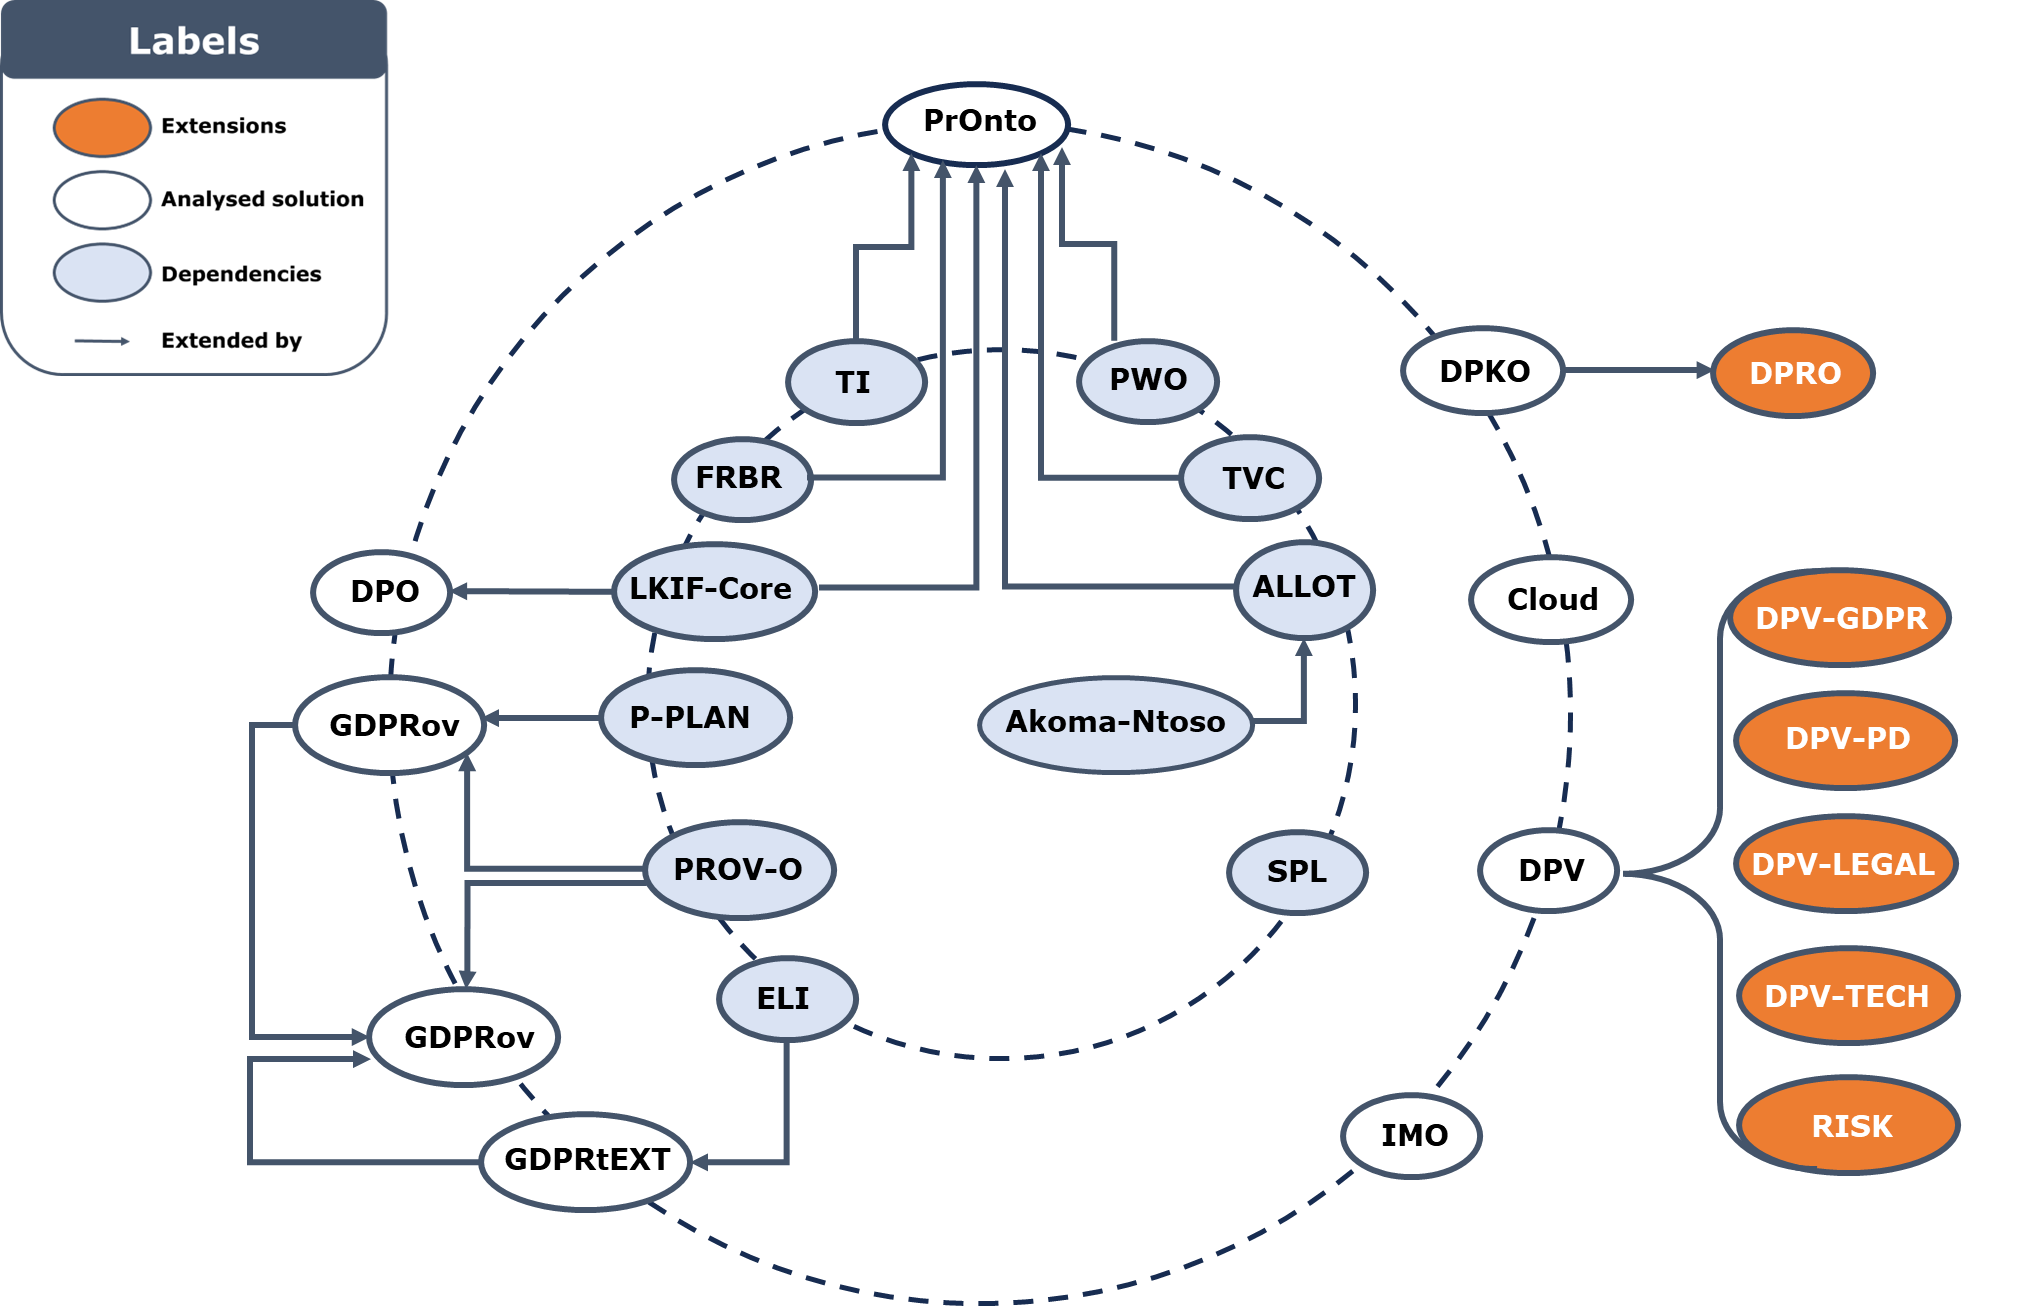
\includegraphics[width=\textwidth]{figures/chapter-2/vocabs.png}
\end{figure}

To complement the description of vocabularies presented in this Section, additional documentation and resources were published in a Web page\footnote{Available at \url{https://protect.oeg.fi.upm.es/sota/ontologies}. Its public repository can be consulted at \url{https://github.com/besteves4/SotAResources} for further improvement when new solutions appear.}, including diagrams and code examples.

\subsubsection{NEURONA}
\label{sec:neurona}

The NEURONA project~\citep{casellas_ontological_2010}, developed by S21SEC\footnote{\url{https://www.s21sec.com/} (accessed on 16 July 2023)} and IDT-UAB\footnote{\url{https://portalrecerca.uab.cat/en/organisations/law-and-technology-institute} (accessed on 16 July 2023)}, created two ontologies based on the pre-GDPR Spanish personal data protection regulation~\citeyearpar{noauthor_real_2008} -- the Data Protection Knowledge Ontology (DPKO) and the Data Protection Reasoning Ontology (DPRO).
These ontologies are, however, not publicly available for re-usage.

The main objectives of the ontologies developed in the context of this project were to represent security measures for files containing personal data and reason over their correctness.
DPKO's main classes are \textbf{data}, \textbf{consent}, \textbf{purpose}, \textbf{person}, \textbf{security measures} and \textbf{security degree}.
In relation to the data class, categories such as health data are defined and associated with special security measures. 
The consent should be given by the data subject in an unambiguous way and for a specific purpose.
In addition, technical and organisational measures (TOMs) for data security, such as access control measures or authentication procedures, are modelled and connected to the nature of the data, taking into consideration the security level associated with the type of data or how the data was obtained. 
For example, a file with health data obtained without consent should have high-level security measures, while a file with anonymised data can implement low-level measures.
DPRO is then used to access data protection compliance by reasoning over the measures applied to files.

\subsubsection{DPO}
\label{sec:dpo}

The Data Protection Ontology (DPO)~\citep{bartolini_reconciling_2015,otake_using_2017} concentrates on the modelling of data protection principles and data controller obligations. It is based on an early version of the GDPR, prior to its implementation in May 2018, on the Data Protection Directive~\citeyearpar{noauthor_directive_1995} and the \textit{Handbook on European data protection law}~\citep{european_union_agency_for_fundamental_rights_and_council_of_europe_handbook_2018} and reuses concepts from the LKIF-Core~\citep{hoekstra_lkif_2007} ontology.

The core classes of DPO are \textbf{data protection principles}, \textbf{rules} for processing and transferring data, and \textbf{data subjects rights}.
The ontology is designed so that each rule and right is linked to at least one principle.
For instance, data subjects have the right to rectify inaccurate or incomplete data, and data controllers must provide the means to do it, according to GDPR's \textit{`accuracy'} principle.
Furthermore, DPO defines consent as a legal justification connected with the principle of trust and also specifies concepts to model the special case of giving consent as a parent for a child, although the concept of \textit{`consent provided by delegation'} is missing.
Data protection-related entities, such as data controllers, supervisory authorities, processors, representatives, or data protection officers, are modelled as a type of \textbf{person}.

Listing \ref{list:sparql_dpo} provides an example of a SPARQL query to retrieve duties of a data controller that do not concern the transfer of personal data using DPO.\footnote{More examples are available in a project repository at \url{https://bitbucket.org/guerret/lu.uni.eclipse.bpmn2/} (accessed on 16/July/2023).}

\begin{listing}[ht]
\caption{SPARQL query to retrieve duties of the data controller that do not concern data transfer using the Data Protection Ontology.}
\label{list:sparql_dpo}
\begin{minted}{sparql}
SELECT DISTINCT ?duty WHERE {
    ?x rdfs:subClassOf* [ rdf:type dpo:Rule ] .
	?x rdfs:label ?duty
	MINUS {
		?x rdfs:subClassOf* [ rdf:type dpo:TransferRule ] .
		?x rdfs:label ?duty .
	} .
	FILTER (?duty != "Rule"@en && ?duty != "ProcessingRule"@en && ?duty != "TransferRule"@en) }
\end{minted}
\end{listing}

\subsubsection{GDPRov}
\label{sec:gdprov}

The GDPR Provenance Ontology (GDPRov)~\citep{pandit_modelling_2017} aims to record the provenance of personal data and of the consent conditions and processing activities performed over such data, according to the GDPR.
GDPRov extends PROV-O~\citep{lebo_prov-o_2013}, a W3C Recommendation created to define the provenance of entities and systems, and P-Plan~\citep{garijo_augmenting_2012}, an extension of PROV-O to represent activities and corresponding steps to execute them, as well as the entities involved.
Using these terms, it is possible to monitor changes in consent or to track the interaction between entities involved in the exchange of data.

GDPRov's main concept to record the provenance of consent is the \textbf{consent agreement template} class, a common template that includes the consent conditions presented to the users and the entities in charge of data processing, and also information on third party sharing, approved processing activities and additional rights.
Provenance metadata on the origin, use, storage, and sharing of the data can also be recorded with GDPRov, as well as information regarding transformations performed to the data.
In addition to this, provenance data on the exercising and fulfilment of GDPR-related rights and obligations can also be represented with GDPRov -- for each right or obligation, a plan can be modelled to include the activities that need to be executed when a user exercises a particular right.

Listing \ref{list:sparql_gdprov} illustrates a SPARQL query that uses GDPRov's terms to retrieve the entities involved in acquiring consent.

\begin{listing}
\caption{SPARQL query retrieving entities involved in acquiring consent using GDPRov~\citep{pandit_modelling_2017}.}
\label{list:sparql_gdprov}
\begin{minted}{sparql}
SELECT ?consent ?template ?toc WHERE {
    ?consent a gdprov:ConsentAgreement .
    ?template a gdprov:ConsentAgreementTemplate .
    ?toc a gdprov:TermsAndConditions .
    ?step a gdprov:ConsentAcquisitionStep .
    ?step gdprov:usesConsentAgreementTemplate ?template .
    ?step gdprov:usesTermsAndConditions ?toc .
    ?step gdprov:generatesConsentAgreement ?consent }
\end{minted}
\end{listing}

\subsubsection{Cloud}
\label{sec:cloud}

The Cloud GDPR ontology was developed by~\cite{elluri_knowledge_2018} to express data protection obligations of cloud data consumers and providers, taking into consideration the Cloud Security Alliance (CSA) controls defined on the \textit{Code of Conduct for GDPR Compliance}~\citep{cloud_security_alliance_-_privacy_level_agreement_working_group_code_2017}.

The \textbf{stakeholders}, \textbf{controls}, and \textbf{obligations} are the core concepts of this ontology.
Cloud-related obligations are extracted and connected to GDPR's articles and are also associated with CSA requirements using the \textbf{hasCSAcontrol} property.
Moreover, these obligations are further specified into common or provider/consumer-specific obligations taking into consideration which stakeholders they are applicable to, e.g., maintaining records of data processing activities and notifying data breaches are common obligations, while providing legal representatives for non-EU stakeholders or hiring a DPO are the responsibility of the consumer and of the provider, respectively.

This work was later extended \citep{elluri_integrated_2018} to automate the implementation of compliance tasks mandated by the GDPR and the Payment Card Industry Data Security Standard (PCI DSS) guidelines~\citep{pci_security_standards_council_payment_2018} and also to include the rights of consumers, providers and end users.
These guidelines deal with financial data, such as the credit card number or card-holder's name, which fall under the protection offered by the GDPR.
As such, and since its scope is narrower, a data breach of PCI DSS-related data automatically results in a GDPR-related one.
Thus, the cloud-related PCI DSS requirements were used to enhance this ontology and its evaluation was performed using privacy policies from five major companies that deal with card-holder's data.

\subsubsection{PrOnto}
\label{sec:pronto}

PrOnto, the Privacy Ontology for legal reasoning, aims to model GDPR-related associations between agents, processing activities, data categories, and deontic modalities, with the main goal to support legal reasoning and compliance with data protection regulations~\citep{ko_pronto_2018}.
PrOnto relies on a number of ontologies to model these relationships:
\begin{itemize}
    \item LKIF-Core~\citep{hoekstra_lkif_2007} is used to model agents, e.g., organisations, software, or people, as well as the several legal roles which can be assigned to them, i.e., acting as data controller or processor.
    \item The Functional Requirements for Bibliographic Records (FRBR) ontology~\citep{byrum_functional_2009} is used to model legal documents as sources of information, that regulate the different relationships between the agents documented in the text, and to register changes in their representation over time. % copied
    \item The ALLOT (A Light Legal Ontology On Top level classes) ontology, developed by~\citep{barabucci_managing_2010}, extends the Akoma Ntoso standard~\citep{palmirani_akoma-ntoso_2011} to link documents with the data they contain, e.g., people, events or locations.
    \item The Publishing Workflow Ontology (PWO)~\citep{gangemi_publishing_2017} is used to characterise provenance data associated with the publication of a document, e.g., to model the different types of processing of personal data.
    \item The TVC (Time-indexed Value in Context) ontology~\citep{peroni_semantic_2014} and the TI (Time Interval) ontology pattern\footnote{\url{http://www.ontologydesignpatterns.org/cp/owl/timeinterval.owl} (accessed on 16/July/2023)} are used to associate time-dependent variables such as events to specific agent roles that only emerge in particular point in time.
\end{itemize}

PrOnto's main classes are defined as follows: \textbf{documents and data}, \textbf{agents and roles}, \textbf{processing and workflow}, \textbf{legal rules and deontic formula}, and \textbf{purposes and legal bases}.
GDPR is the main document used to extract personal data categories such as judicial or sensitive data and non-personal data such as anonymous or legal person data.
Moreover, processing activities are represented as a workflow of actions that should be recorded together with provenance data such as the context and time in which each action occurs.
Each processing activity is also associated with a purpose and a legal rule, which is composed of deontic specifications, i.e., prohibitions, rights, permissions, and obligations, used to check if the activity being executed is compliant with the GDPR. PrOnto is, however, not publicly available for re-usage, which hinders the assessment of the totality of concepts it models\footnote{As PrOnto is not available online, its namespace is unknown. In this Thesis, the prefix \texttt{pronto} is used to identify PrOnto's concepts that are available in the analysed publication.}. 

Listing \ref{list:sparql_pronto} illustrates a query to retrieve information regarding personal data processing activities performed by company \textit{X} in the role of controller from time \textit{t1} to \textit{t2}.

\begin{listing}[ht]
\caption{SPARQL query used to retrieve personal data processing activities performed by company \textit{X} in the role of controller from \textit{t1} to \textit{t2} using PrOnto~\citep{ko_pronto_2018}.}
\label{list:sparql_pronto}
\begin{minted}{sparql}
SELECT ?pdp WHERE {
    ?pdp pronto:isManagedBy _:c .
    [ lkif:plays _:c ;
        rdfs:label "X" ] .
    ?pdp pronto:isValid [
        ti:hasIntervalStartDate [ 
            a ti:TimeInterval; rdfs:label "t1" ] ;
        ti:hasIntervalEndDate [ 
            a ti:TimeInterval; rdfs:label "t2" ] ] . }
\end{minted}
\end{listing}

\subsubsection{GConsent}
\label{sec:gconsent}

GConsent \citep{hitzler_gconsent_2019} is an ontology focused on the GDPR concept of consent and, as such, it models information regarding how consent was collected and stored, as well as records of any changes that may occur over time, including withdrawal, including data on the parties involved, according to Article 6 of the GDPR.
Additionally, other documentation sources were also adopted, including EDPB's guidelines on consent~\citep{european_data_protection_board_guidelines_2020}.
GConsent encompasses not just the notion of consent, but also depicts its status, context, and origin.
To achieve this, it leverages established vocabularies in this domain, including PROV-O~\citep{lebo_prov-o_2013}, GDPRov~\citep{pandit_modelling_2017}, and GDPRtEXT~\citep{gangemi_gdprtext_2018} (discussed in Section~\ref{sec:gdprtext}).

GConsent's main concepts are the terms to represent \textbf{data subjects}, \textbf{personal data}, \textbf{purpose} and \textbf{processing types}, as well as the \textbf{consent} and \textbf{consent status} classes -- the latter fills a gap on the available ontologies on this domain as it not only defines \textbf{explicitly given consent} as a concept, but also classifies other states of consent, such as \textbf{implicitly given}, \textbf{expired} or \textbf{refused}.
GConsent also includes concepts to represent information regarding the context in which the consent was obtained -- information about the entities involved, spatial and temporal aspects, and the format used to record it, e.g., Web form, voice recording, or signature -- and a taxonomy of processing types, e.g., data alignment or data retrieval.

Listing \ref{list:ttl_gconsent} provides an example of a record of provenance data regarding an activity of withdrawing consent using GConsent.

\begin{listing}[ht]
\caption{Turtle record of provenance data regarding an activity of withdrawing consent using GConsent \citep{hitzler_gconsent_2019}.}
\label{list:ttl_gconsent}
\begin{minted}{turtle}
ex:modifyConsent a gdprov:ModifyConsentActivity ;
    prov:invalidated ex:consent1 ;
    prov:generated ex:consent2 .

ex:consent1 a gc:Consent ;
    gc:isPreviousConsentFor ex:consent2 ;
    gc:hasStatus gc:ConsentStatusExplicitlyGiven .

ex:consent2 a gc:Consent ;
    gc:hasStatus gc:ConsentStatusWithdrawn .
\end{minted}
\end{listing}

\subsubsection{IMO}
\label{sec:imo}

The Information Model Ontology (IMO)~\citep{papagiannakopoulou_leveraging_2014,lioudakis_compliance_2019} was developed in the context of the BPR4GDPR project\footnote{BPR4GDPR (Business Process Re-engineering and functional toolkit for GDPR compliance) is an European Union H2020 innovation programme with the main goal of providing a framework to reinforce the implementation of GDPR-compliant measures inside organisations at diverse scales and in several domains. More information available at \url{https://www.bpr4gdpr.eu/} (accessed on 16/July/2023).} and it aims to define the entities and respective roles that are involved in the organisation lifecycle of processing personal data.


IMO's main concepts encompass various categories: \textbf{data types}, \textbf{roles} across diverse organisational structures, \textbf{machine types} housing \textbf{operations} tailored for specific \textbf{purposes}, \textbf{events} alongside their contextual details.
The roles class specifically pertains to the duties assigned to users within organisational contexts, with the potential for hierarchical implementations based on the granularity of data.
Data processing activities are represented via the operations class, which is equipped with the \textbf{hasInput} and \textbf{hasOutput} properties.
These properties facilitate the connection between operations and the data being processed, as well as the resulting data and their corresponding states, e.g., normal or anonymised form.
These operations can be organised within an operation container, a concept designed to group processing activities that typically function together within specific contexts.
For example, within database management, functions such as create, read, update, or delete are frequently employed together.
Instances of the role and operation classes are consistently linked with a purpose instance.
Moreover, the events class, designed to encompass all processing activities such as data breaches or consent withdrawals, should be paired with the context class to create specific event instances with temporal and spatial details, among other pertinent information.

% TODO: extract example from https://www.researchgate.net/profile/Joaquin-Garcia-Alfaro/publication/260706010/figure/fig3/AS:296857856167938@1447787836426/Example-of-Ontological-Access-Control-Rule.png
\begin{listing}
\caption{Turtle record of a personal data handling related to the collection and usage of email addresses for marketing purposes using DPV~\citep{panetto_creating_2019}.}
\label{list:ttl_dpv}
\begin{minted}{turtle}
ex:PDHforMarketing a dpv:PersonalDataHandling ;
    dpv:hasDataController [ a dpv:DataController ] ;
    dpv:hasPersonalData dpv-pd:EmailAddress ;
    dpv:hasProcessing dpv:Collect, dpv:Use ;
    dpv:hasPurpose dpv:Marketing .
\end{minted}
\end{listing}

\subsubsection{DPV}
\label{sec:dpv}

The Data Privacy Vocabulary is being developed and maintained by the W3C Data Protection Vocabularies and Controls Community Group (DPVCG)\footnote{\url{https://www.w3.org/community/dpvcg/} (accessed on 16/July/2023)} -- an output of a W3C workshop on data privacy controls which took place in 2018, with the objective of defining priorities for the standardisation of this domain~\citep{bonatti_data_2018}.

DPV's core concepts, \textbf{processing}, \textbf{purpose}, \textbf{recipient} and \textbf{personal data categories}, were adapted from the SPECIAL Usage Policy Language (SPL) vocabularies~\citep{bonatti_policy_2018} and new concepts were/are continuously added to DPV after being discussed and agreed upon by the Community Group.
In addition to previously mentioned concepts, DPV's base vocabulary was first published with the following additional classes: \textbf{legal basis}, \textbf{technical and organizational measures} and \textbf{legal entities}, including \textbf{data subject} and \textbf{child}, \textbf{recipients}, \textbf{data controller}, \textbf{data processor} and \textbf{third party}~\citep{panetto_creating_2019}.
In December of 2022, DPV version 1 was published including additional concepts to model \textbf{risk}, \textbf{rights} and \textbf{data subject rights}, \textbf{technology}, \textbf{laws} and \textbf{context of processing} classes and the previously existing taxonomies were extended with new terms -- new legal entities, including authority and data protection authority, vulnerable data subject, data sub-processor, data protection officer and representative, were added to the vocabulary, as well as new purpose and legal basis sub-classes.
For instance, the purpose taxonomy is composed of 76 purpose sub-classes, which are topped by classes such as R\&D or Service Provision, and can be further constrained to specific contexts or business sectors, and DPV's processing operations taxonomy covers the terms defined in Article 4.2 of the GDPR, providing a set of 44 processing categories.

DPV also provides five extensions:
\begin{itemize}
    \item Personal data categories are defined in the DPV-PD extension\footnote{\url{https://w3id.org/dpv/dpv-pd} (accessed on 17/July/2023)} -- the personal data class is split into generic classes such as financial or social data, adapted from the \textbf{EnterPrivacy} taxonomy by \cite{cronk_categories_2017}, which are further specified into concepts such as credit card number or social media accounts.
    \item GDPR-specific concepts are defined in the DPV-GDPR extension\footnote{\url{https://w3id.org/dpv/dpv-gdpr} (accessed on 17/July/2023)} -- it covers legal bases specified on GDPR's Articles 6 and 9 for the processing of personal data and also the legal bases for the transfer of personal data to third countries defined on Articles 45, 46 and 49. It also models GDPR's data subject rights, data transfer tools and Data Protection Impact Assessment (DPIA) terms.
    \item Technology-relevant concepts are defined in the DPV-TECH extension\footnote{\url{https://w3id.org/dpv/dpv-tech} (accessed on 17/July/2023)} -- it includes concepts to model specific technologies, their management, technology actors, and relevant tools and systems.
    \item Jurisdiction-relevant concepts are defined in the DPV-LEGAL extension\footnote{\url{https://w3id.org/dpv/dpv-legal} (accessed on 17/July/2023)} -- it contains terms related to specific laws, adequacy decisions and a taxonomy of authorities.
    \item Risk concepts are defined in the RISK extension\footnote{\url{https://w3id.org/dpv/risk} (accessed on 17/July/2023)} -- it covers concepts related to risk, likelihood, severity levels, consequences and impacts, as well as risk assessment techniques and methodologies.
\end{itemize}

Listing \ref{list:ttl_dpv} provides an example of a personal data handling related to the collection and usage of email addresses for marketing purposes using DPV.

\begin{listing}[ht]
\caption{Turtle record of a personal data handling related to the collection and usage of email addresses for marketing purposes using DPV~\citep{panetto_creating_2019}.}
\label{list:ttl_dpv}
\begin{minted}{turtle}
ex:PDHforMarketing a dpv:PersonalDataHandling ;
    dpv:hasDataController [ a dpv:DataController ] ;
    dpv:hasPersonalData pd:EmailAddress ;
    dpv:hasProcessing dpv:Collect, dpv:Use ;
    dpv:hasPurpose dpv:Marketing .
\end{minted}
\end{listing}

\subsubsection{GDPRtEXT}
\label{sec:gdprtext}

GDPRtEXT was developed by~\cite{gangemi_gdprtext_2018} as a linked data resource, which extends the European Legislation Identifier (ELI) ontology~\citep{office_of_publications_on_eur-lex_eu_2017}, to connect GDPR concepts with the specific chapters, articles or points of the regulatory text.

The main concepts modelled in this ontology are related to the specific \textbf{entities} mentioned in the GDPR text, their \textbf{rights} and \textbf{obligations}, the \textbf{principles} and the \textbf{activities} which specify processes and actions defined in the GDPR, such as reporting a data breach, exercising rights or demonstrating consent.
These terms are linked to the relevant GDPR articles using the \texttt{rdfs:isDefinedBy} property.

\subsection{Comparative analysis}
\label{sec:sota_vocabularies_analysis}

% TODO: \beatriz{DPKO: I7 - only consent; I17 - data}
% TODO: \beatriz{DPKO: I20 - transfer rule}

As it is visible in Tables \ref{tab:vocabsTerms-first} and \ref{tab:vocabsTerms-second}, existing ontologies and vocabularies in the domain of data protection are of particular interest to represent the privacy terms described in Table~\ref{tab:GDPR_privacy_terms}, however, there are still representational gaps to be filled.
More specifically, each ontology was analysed in terms of the concepts they model and, when a particular concept was found to represent a particular privacy term, the name of the respective term was included in the comparative tables, as well as the number of sub-classes which can be used to more precisely define the term.
The cases in which there was no specific concept to represent the privacy term, yet there were terms that can be extended to accomplish it, are marked with an asterisk. % copied
Privacy terms I15, I19, I24, I26, and I28 to I30 are not represented in either Table~\ref{tab:vocabsTerms-first} or~\ref{tab:vocabsTerms-second} since they are not modelled by any of the analysed ontologies. % copied

DPO, GDPRov, PrOnto, DPV and GDPRtEXT can be used to partially populate a great deal of the informational items required by the \textit{`right to be informed'} and the other GDPR rights. % copied
However, DPV and GDPRtEXT must be highlighted since they contain the concepts to represent, at least partially, 19 and 14 privacy terms, respectively, out of the 30 described in Table~\ref{tab:GDPR_privacy_terms}.
Furthermore, these vocabularies are the ones that have the largest number of sub-classes to specifically define the respective terms. % copied

Of particular importance, it must be referred that most of presented resources are obsolete or without new developments in recent years, with DPV being the only one that presented new outcomes in the last two years.
Moreover, of all the covered vocabularies, only DPKO, IMO and PrOnto do not have open and accessible resources. % copied

\begin{table}
\centering
\caption[Representation of privacy terms I1 to I22 in the DPKO, DPRO, DPO, GDPRov, Cloud and PrOnto ontologies.]{Representation of privacy terms I1 to I22 in the DPKO, DPRO, DPO, GDPRov, Cloud and PrOnto ontologies. The names of the classes which can be used to specify a particular item are depicted in the table, as well as their respective number of sub-classes, if available. The privacy terms which can not be fully represented by the current ontology terms are illustrated with an asterisk.}
\label{tab:vocabsTerms-first}
\resizebox{\textwidth}{!}{%
\begin{tabular}{ c||c|c|c|c|c|c}
 & DPKO & DPRO & DPO & GDPRov & Cloud & PrOnto \\
 \hline\hline
 I1 & & & Controller & Controller & & $\ast$ \\
 \hline
 I3 & & & & ControllerRepresentative & Identify\_Representatives & \\
 \hline
 I6 & Purpose & & Purpose & & & Purpose (10) \\
 \hline
 I7 & $\ast$ & & LegalJustification (6) & & & \\
 \hline
 I8 & & & LegitimateInterest & & & \\
 \hline
 I9 & & & Recipient (2) & & & $\ast$ \\
 \hline
 I10 & & & & $\ast$ & & \\
  \hline
 I11 & & & & & & $\ast$ \\
 \hline
 I12 & & & DataSubjectRight (7) & Process (10) & & Right (8) \\
 \hline
 I16 & & & AutomatedProcessing & $\ast$ & & \\
 \hline
 I17 & $\ast$ & & PersonalData & PersonalData (3) & & PersonalData (7) \\
 \hline
 I20 & & & $\ast$ & & & \\
 \hline
 I21 & & & & ProvideCopyOfPersonalData & & \\
 \hline
 I22 & & & & RectifyData & & \\
\end{tabular}}
\end{table}

\begin{table}
\centering
\caption[Representation of privacy terms I1 to I27 in the GConsent, IMO, DPV and GDPRtEXT ontologies.]{Representation of privacy terms I1 to I27 in the GConsent, IMO, DPV and GDPRtEXT ontologies. The names of the classes which can be used to specify a particular item are depicted in the table, as well as their respective number of sub-classes, if available. The privacy terms which can not be fully represented by the current ontology terms are illustrated with an asterisk.}
\label{tab:vocabsTerms-second}
\resizebox{\textwidth}{!}{%
\begin{tabular}{ c||c|c|c||c}
 & GConsent & IMO & DPV & GDPRtEXT \\
 \hline\hline
 I1 & DataController & DataController & DataController & Controller \\
 \hline
 I2 & & & hasContact & \\ 
 \hline
 I3 & & & Representative & ControllerRepresentative \\
 \hline
 I4 & & & hasContact & \\ 
 \hline
 I5 & & & hasContact & \\ 
 \hline
 I6 & Purpose & Purposes & Purpose (76) & \\
 \hline
 I7 & $\ast$ & & LegalBasis (26) & LawfulBasisForProcessing (14) \\
 \hline
 I8 & & & A6-1-f & LegitimateInterest \\
 \hline
 I9 & $\ast$ & & Recipient (4) & $\ast$ \\
 \hline
 I10 & & & $\ast$ & CrossBorderTransfer \\
 \hline
 I11 & $\ast$ & $\ast$ & $\ast$ & RecordDataRetentionPeriod \\
 \hline
 I12 & & & DataSubjectRight (12) & Rights (10) \\
 \hline
 I13 & $\ast$ & & A7-3 & \\
 \hline
 I14 & & & A77 & \\
 \hline
 I16 & & & AutomatedDecisionMaking & AutomatedProcessing \\
 \hline
 I17 & & DataTypes (52) & PersonalData (206) & PersonalData (5) \\
 \hline
 I18 & & & DataSource & InfoAboutSourceOfData \\ 
 \hline
 I20 & & & $\ast$ & \\
 \hline
 I21 & & & & ProvideCopyOfPersonalData \\
 \hline
 I23 & & & & RightOfErasure (2) \\
 \hline
 I25 & & & hasContact & \\ 
 \hline
 I27 & & & & RightToRestrictProcessing (3) \\
\end{tabular}}
\end{table}